\chapter{АНАЛИЗ ПРЕДМЕТНОЙ ОБЛАСТИ РЕКОМЕНДАТЕЛЬНЫХ СИСТЕМ}
\label{chap:analysis}
\aftertitle

\section{Понятие рекомендательных систем}

Задача фильтрации новостей и сообщений в групповых чатах решается рекомендательными системами. Рекомендательная система ~--  программная система, которая пытается предсказать, какие объекты (фильмы, музыка, книги, новости, веб-сайты) будут интересны пользователю, имея определенную информацию о его профиле \cite{recommendation_system_wiki}.

Существует несколько традиционных подходов к построению рекомендательных систем \cite{recommendation_system_methods}: контент-ориентированный подход и коллаборативная фильтрация.

Суть контент-ориентированного подхода заключается в сопоставлении аттрибутов контента и пользователей. Например, здесь могут быть использованы категориальные аттрибуты (жанр фильма, актеры фильма и т.п.), числовые аттрибуты (продолжительность, рейтинг и т.п.) для составления эмбеддингов или вектора предмета ~-- векторных представлений объекта рекомендации. Аналогично составляется вектор пользователя. Построив эмбеддинги пользователя и объектов, можно осуществлять рекомендации. Объект рекомендуется пользователю, если его эмбеддинги близки к эмбеддингам пользователя, либо к эмбеддингам других объектов, купленных (просмотренных, прочитанных и т.п.) пользователем.

В качестве эмбеддингов могут выступать и различные текстовые описания. В классических рекомендательных системах могут использоваться такие методы, как TF-IDF \cite{no-patterns}, а в современных рекомендательных системах ~-- текстовые эмбеддинги, полученные с помощью больших языковых моделей \cite{tf_augumenting_recommendation}.

В последнее время активно развиваются подходы с использованием больших языковых моделей в рекомендательных системах.

\section{Развитие методов обработки естественного языка}

Большая языковая модель (Large Language Model, LLM) ~-- искусственная нейронная сеть, предназначенная для обработки и понимания естественного языка (natural language processing).

Языковые модели являются одним из способов решения задач обработки естественного языка и генерации текста. Языковые модели моделируют естественный язык путем генерации следующих или пропущенных слов в текстовых последовательностях. Развитие языковых моделей можно разделить на следующие этапы: статистические модели, базовые нейросетевые модели, предобученные модели и большие языковые модели \cite{llm_survey}. Эти этапы развития языковых моделей представлены на рисунке \ref{img:llm_evolution}.

\begin{figure}[h]
    \centering
    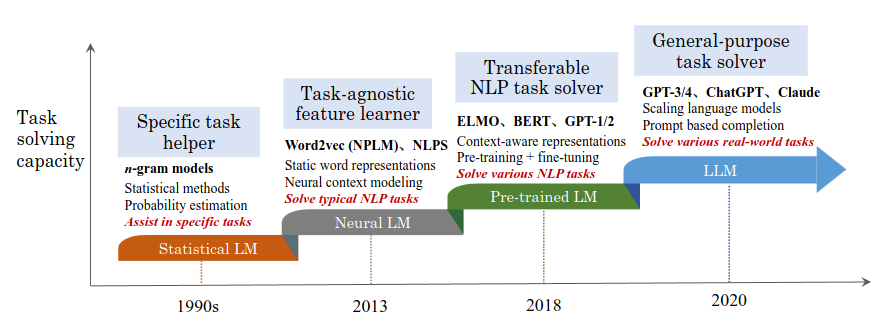
\includegraphics[width=\linewidth]{../images/llm_evolution.png}
    \caption{Развитие языковых моделей с точки зрения объема решаемых задач\cite{llm_survey}}
    \label{img:llm_evolution}
\end{figure}

Статистические модели основаны на классических методах машинного обучения и статистики. Типичным подходом к языковому моделированию являлось использованием марковских цепей для предсказания следующих элементов последовательности. Такие модели, имеющие фиксированный контекст из нескольких предыдущих элементов, называются n-gram моделями.

Следующим шагом в развитии языковых моделей стало использование искусственных нейронных сетей (сетей прямого распространения и рекуррентных нейронных сетей). Важным шагом стало создание векторных представлений слов (эмбеддингов), таких как word2vec \cite{word2vec}. Этот метод позволяет представлять слова текста в виде векторов, близость которых отражает семантическую близость слов. Подход word2vec основан на гипотезе локальности, которая утверждает, что слова, которые встречаются в одинаковых окружениях, имеют близкие значения. Этот и подобные методы продемонстрировали высокую эффективность в различных задачах обработки естественного языка. Подход с использованием нейронных сетей, в основном, рекуррентных нейронных сетей RNN и LSTM, позволил реализовать end-to-end модели, решающие различные типичные задачи обработки естественного языка.

Дальнейшим развитием этих принципов стали предобученные языковые модели. В отличие от word2vec, который обучается независимым от контекста представлениям, языковые модели способны понимать значение слова с учетом окружающего контекста.

Первой попыткой создания контекстуальных эмбеддингов стал Elmo \cite{elmo}. Эта модель способна запоминать представления слов, зависящие от контекста. Эта модель основана на архитектуре двусторонней LSTM.

Важным шагом в развитии моделей обработки естесственного языка и в целом последовательностей стало появление архитектуры Трансформер \cite{transformer}. Трансформер представляет собой sequence-to-sequence модель, преобразующую текст (последовательность токенов) в другую последовательность токенов. Архитектурно он состоит из стека энкодеров, которые кодируют последовательность в некое внутреннее представление, и стека декодеров, которые генерируют новую последовательность. Важнейшим компонентом архитектуры Трансформера является механизм внимания (attention). Это механизм, который позволяет определять взаимную значимость токенов в последовательности, тем самым, позволяя лучше выстраивать связи между токенами (словами), которые расположены далеко друг от друга. Ключевым вкладом архитектуры Трансформера был отказ от использования рекуррентных нейронных сетей и использование только лишь механизма внимания. Это позволило существенно улучшить вычислительную производительность модели и ее возможность к удержанию большого контекста, что, в свою очередь, дало возможным создавать большие модели, состоящие из десятков миллиардов параметров, что было бы невозможно с использованием рекуррентных нейронных сетей.

С тех пор, архитектура Трансформер является основной архитектурой всех новейших state-of-the-art моделей по обработке естественного языка. На основе Трансформера были созданы такие получившие широкое распространение архитектуры как BERT \cite{bert} и GPT \cite{gpt}.

Важной особенностью этих моделей является возможность использования трансферного обучения (transfer learning). Трансферное обучение ранее широко применялось в задачах компьютерного зрения. Суть данного метода заключается в использовании базовой модели, называемой backbone, которая обучена на большом количестве общих данных, которая затем до-обучается на конкретных данных, специфичных для решаемой задачи. Это техника позволяет использовать очень глубокие нейронные сети, которые требуют большой объем обучающих данных и значительные вычислительные ресурсы для обучения.

Языковые модели обучаются с помощью техники self-supervised learning. Существуют различные методики обучения, такие как MLM (masked language modeling), CLM (casual language modeling) и др. В случае MLM некоторые слова (токены) в тексте заменяются на маску, задачей модели является предсказать закрытый токен. В случае CLM задачей модели является предсказать следующий токен последовательности. Это является ключевой частью успеха языковых моделей. Качество решения задач на естественном языке зависит от размера модели (количества параметров) и от объема обучающей выборке. Используемых подход позволяет обучать модели на очень больших объемах текстовой информации без необходимости в ручной разметке данных.

Обученная на большом корпусе текстов языковая модель может выступать в качестве базовой модели для построения различных моделей для решения специфичных задач, таких как определение тональности текста, фильтрация текста, чат-боты и рекомендательные системы.

Следующим шагом развития моделей обработки естественного языка стало появление больших языковых моделей. Было обнаружено, что с ростом размера модели (количества параметров) и объема обучающей выборки, результаты моделей улучшаются. Более того, большие модели показали качественно отличное поведение от моделей меньшего размера. C определенного размера модели происходит значительный нелинейный рост производительности моделей в различных задачах. Данное явление было названо эмерджентным поведением \cite{llm_emergent}. Зависимость метрик в различных задачах обработки естественного языка от количества параметров модели представлена на рисунке \ref{img:llm_scaling}.

\begin{figure}[h]
    \centering
    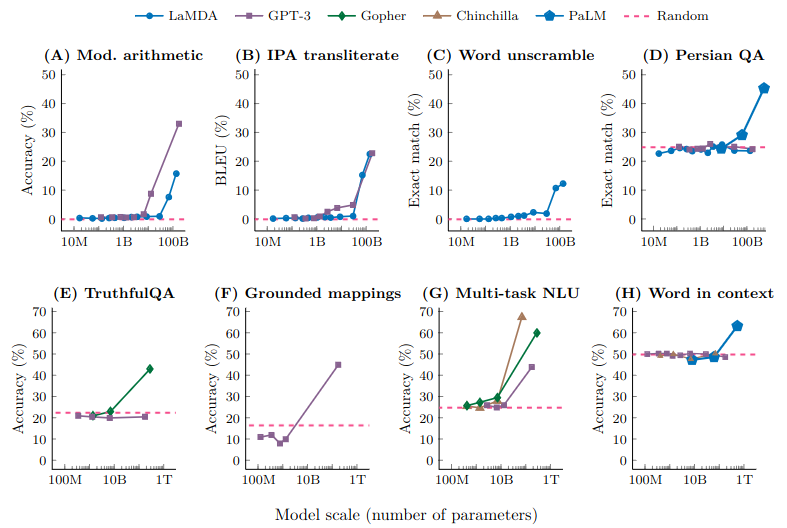
\includegraphics[width=\linewidth]{../images/llm_scaling.png}
    \caption{Зависимость метрик в различных задачах обработки естественного языка от количества параметров модели \cite{llm_emergent}}
    \label{img:llm_scaling}
\end{figure}
